%% bare_jrnl_compsoc.tex
%% V1.4b
%% 2015/08/26
%% by Michael Shell
%% See:
%% http://www.michaelshell.org/
%% for current contact information.
%%
%% This is a skeleton file demonstrating the use of IEEEtran.cls
%% (requires IEEEtran.cls version 1.8b or later) with an IEEE
%% Computer Society journal paper.
%%
%% Support sites:
%% http://www.michaelshell.org/tex/ieeetran/
%% http://www.ctan.org/pkg/ieeetran
%% and
%% http://www.ieee.org/

%%*************************************************************************
%% Legal Notice:
%% This code is offered as-is without any warranty either expressed or
%% implied; without even the implied warranty of MERCHANTABILITY or
%% FITNESS FOR A PARTICULAR PURPOSE! 
%% User assumes all risk.
%% In no event shall the IEEE or any contributor to this code be liable for
%% any damages or losses, including, but not limited to, incidental,
%% consequential, or any other damages, resulting from the use or misuse
%% of any information contained here.
%%
%% All comments are the opinions of their respective authors and are not
%% necessarily endorsed by the IEEE.
%%
%% This work is distributed under the LaTeX Project Public License (LPPL)
%% ( http://www.latex-project.org/ ) version 1.3, and may be freely used,
%% distributed and modified. A copy of the LPPL, version 1.3, is included
%% in the base LaTeX documentation of all distributions of LaTeX released
%% 2003/12/01 or later.
%% Retain all contribution notices and credits.
%% ** Modified files should be clearly indicated as such, including  **
%% ** renaming them and changing author support contact information. **
%%*************************************************************************


% *** Authors should verify (and, if needed, correct) their LaTeX system  ***
% *** with the testflow diagnostic prior to trusting their LaTeX platform ***
% *** with production work. The IEEE's font choices and paper sizes can   ***
% *** trigger bugs that do not appear when using other class files.       ***                          ***
% The testflow support page is at:
% http://www.michaelshell.org/tex/testflow/


\documentclass[12pt,journal,compsoc]{IEEEtran}
\usepackage[margin=1in]{geometry}

%
% If IEEEtran.cls has not been installed into the LaTeX system files,
% manually specify the path to it like:
% \documentclass[10pt,journal,compsoc]{../sty/IEEEtran}


\newenvironment{subs}
  {\adjustwidth{1em}{0pt}}
  {\endadjustwidth}

% Some very useful LaTeX packages include:
% (uncomment the ones you want to load)


% *** MISC UTILITY PACKAGES ***
%
%\usepackage{ifpdf}
% Heiko Oberdiek's ifpdf.sty is very useful if you need conditional
% compilation based on whether the output is pdf or dvi.
% usage:
% \ifpdf
%   % pdf code
% \else
%   % dvi code
% \fi
% The latest version of ifpdf.sty can be obtained from:
% http://www.ctan.org/pkg/ifpdf
% Also, note that IEEEtran.cls V1.7 and later provides a builtin
% \ifCLASSINFOpdf conditional that works the same way.
% When switching from latex to pdflatex and vice-versa, the compiler may
% have to be run twice to clear warning/error messages.


% *** CITATION PACKAGES ***
%
\ifCLASSOPTIONcompsoc
  % IEEE Computer Society needs nocompress option
  % requires cite.sty v4.0 or later (November 2003)
  \usepackage[nocompress]{cite}
\else
  % normal IEEE
  \usepackage{cite}
\fi
% cite.sty was written by Donald Arseneau
% V1.6 and later of IEEEtran pre-defines the format of the cite.sty package
% \cite{} output to follow that of the IEEE. Loading the cite package will
% result in citation numbers being automatically sorted and properly
% "compressed/ranged". e.g., [1], [9], [2], [7], [5], [6] without using
% cite.sty will become [1], [2], [5]--[7], [9] using cite.sty. cite.sty's
% \cite will automatically add leading space, if needed. Use cite.sty's
% noadjust option (cite.sty V3.8 and later) if you want to turn this off
% such as if a citation ever needs to be enclosed in parenthesis.
% cite.sty is already installed on most LaTeX systems. Be sure and use
% version 5.0 (2009-03-20) and later if using hyperref.sty.
% The latest version can be obtained at:
% http://www.ctan.org/pkg/cite
% The documentation is contained in the cite.sty file itself.
%
% Note that some packages require special options to format as the Computer
% Society requires. In particular, Computer Society  papers do not use
% compressed citation ranges as is done in typical IEEE papers
% (e.g., [1]-[4]). Instead, they list every citation separately in order
% (e.g., [1], [2], [3], [4]). To get the latter we need to load the cite
% package with the nocompress option which is supported by cite.sty v4.0
% and later. Note also the use of a CLASSOPTION conditional provided by
% IEEEtran.cls V1.7 and later.


% *** GRAPHICS RELATED PACKAGES ***
%
\usepackage[latin1]{inputenc}
\usepackage{tikz}
\usetikzlibrary{shapes,arrows, positioning, fit, calc}
\usepackage{changepage}


\ifCLASSINFOpdf
  \usepackage[pdftex]{graphicx}
  % declare the path(s) where your graphic files are
  \graphicspath{{./images/}}
  % and their extensions so you won't have to specify these with
  % every instance of \includegraphics
  % \DeclareGraphicsExtensions{.pdf,.jpeg,.png}
\else
  % or other class option (dvipsone, dvipdf, if not using dvips). graphicx
  % will default to the driver specified in the system graphics.cfg if no
  % driver is specified.
  % \usepackage[dvips]{graphicx}
  % declare the path(s) where your graphic files are
  % \graphicspath{{../eps/}}
  % and their extensions so you won't have to specify these with
  % every instance of \includegraphics
  % \DeclareGraphicsExtensions{.eps}
\fi
% graphicx was written by David Carlisle and Sebastian Rahtz. It is
% required if you want graphics, photos, etc. graphicx.sty is already
% installed on most LaTeX systems. The latest version and documentation
% can be obtained at: 
% http://www.ctan.org/pkg/graphicx
% Another good source of documentation is "Using Imported Graphics in
% LaTeX2e" by Keith Reckdahl which can be found at:
% http://www.ctan.org/pkg/epslatex
%
% latex, and pdflatex in dvi mode, support graphics in encapsulated
% postscript (.eps) format. pdflatex in pdf mode supports graphics
% in .pdf, .jpeg, .png and .mps (metapost) formats. Users should ensure
% that all non-photo figures use a vector format (.eps, .pdf, .mps) and
% not a bitmapped formats (.jpeg, .png). The IEEE frowns on bitmapped formats
% which can result in "jaggedy"/blurry rendering of lines and letters as
% well as large increases in file sizes.
%
% You can find documentation about the pdfTeX application at:
% http://www.tug.org/applications/pdftex





% *** MATH PACKAGES ***
%
%\usepackage{amsmath}
% A popular package from the American Mathematical Society that provides
% many useful and powerful commands for dealing with mathematics.
%
% Note that the amsmath package sets \interdisplaylinepenalty to 10000
% thus preventing page breaks from occurring within multiline equations. Use:
%\interdisplaylinepenalty=2500
% after loading amsmath to restore such page breaks as IEEEtran.cls normally
% does. amsmath.sty is already installed on most LaTeX systems. The latest
% version and documentation can be obtained at:
% http://www.ctan.org/pkg/amsmath





% *** SPECIALIZED LIST PACKAGES ***
%
%\usepackage{algorithmic}
% algorithmic.sty was written by Peter Williams and Rogerio Brito.
% This package provides an algorithmic environment fo describing algorithms.
% You can use the algorithmic environment in-text or within a figure
% environment to provide for a floating algorithm. Do NOT use the algorithm
% floating environment provided by algorithm.sty (by the same authors) or
% algorithm2e.sty (by Christophe Fiorio) as the IEEE does not use dedicated
% algorithm float types and packages that provide these will not provide
% correct IEEE style captions. The latest version and documentation of
% algorithmic.sty can be obtained at:
% http://www.ctan.org/pkg/algorithms
% Also of interest may be the (relatively newer and more customizable)
% algorithmicx.sty package by Szasz Janos:
% http://www.ctan.org/pkg/algorithmicx




% *** ALIGNMENT PACKAGES ***
%
\usepackage{array}
% Frank Mittelbach's and David Carlisle's array.sty patches and improves
% the standard LaTeX2e array and tabular environments to provide better
% appearance and additional user controls. As the default LaTeX2e table
% generation code is lacking to the point of almost being broken with
% respect to the quality of the end results, all users are strongly
% advised to use an enhanced (at the very least that provided by array.sty)
% set of table tools. array.sty is already installed on most systems. The
% latest version and documentation can be obtained at:
% http://www.ctan.org/pkg/array


% IEEEtran contains the IEEEeqnarray family of commands that can be used to
% generate multiline equations as well as matrices, tables, etc., of high
% quality.




% *** SUBFIGURE PACKAGES ***
%\ifCLASSOPTIONcompsoc
%  \usepackage[caption=false,font=footnotesize,labelfont=sf,textfont=sf]{subfig}
%\else
%  \usepackage[caption=false,font=footnotesize]{subfig}
%\fi
% subfig.sty, written by Steven Douglas Cochran, is the modern replacement
% for subfigure.sty, the latter of which is no longer maintained and is
% incompatible with some LaTeX packages including fixltx2e. However,
% subfig.sty requires and automatically loads Axel Sommerfeldt's caption.sty
% which will override IEEEtran.cls' handling of captions and this will result
% in non-IEEE style figure/table captions. To prevent this problem, be sure
% and invoke subfig.sty's "caption=false" package option (available since
% subfig.sty version 1.3, 2005/06/28) as this is will preserve IEEEtran.cls
% handling of captions.
% Note that the Computer Society format requires a sans serif font rather
% than the serif font used in traditional IEEE formatting and thus the need
% to invoke different subfig.sty package options depending on whether
% compsoc mode has been enabled.
%
% The latest version and documentation of subfig.sty can be obtained at:
% http://www.ctan.org/pkg/subfig




% *** FLOAT PACKAGES ***
\usepackage{float}
% \usepackage{fixltx2e}
% fixltx2e, the successor to the earlier fix2col.sty, was written by
% Frank Mittelbach and David Carlisle. This package corrects a few problems
% in the LaTeX2e kernel, the most notable of which is that in current
% LaTeX2e releases, the ordering of single and double column floats is not
% guaranteed to be preserved. Thus, an unpatched LaTeX2e can allow a
% single column figure to be placed prior to an earlier double column
% figure.
% Be aware that LaTeX2e kernels dated 2015 and later have fixltx2e.sty's
% corrections already built into the system in which case a warning will
% be issued if an attempt is made to load fixltx2e.sty as it is no longer
% needed.
% The latest version and documentation can be found at:
% http://www.ctan.org/pkg/fixltx2e


%\usepackage{stfloats}
% stfloats.sty was written by Sigitas Tolusis. This package gives LaTeX2e
% the ability to do double column floats at the bottom of the page as well
% as the top. (e.g., "\begin{figure*}[!b]" is not normally possible in
% LaTeX2e). It also provides a command:
%\fnbelowfloat
% to enable the placement of footnotes below bottom floats (the standard
% LaTeX2e kernel puts them above bottom floats). This is an invasive package
% which rewrites many portions of the LaTeX2e float routines. It may not work
% with other packages that modify the LaTeX2e float routines. The latest
% version and documentation can be obtained at:
% http://www.ctan.org/pkg/stfloats
% Do not use the stfloats baselinefloat ability as the IEEE does not allow
% \baselineskip to stretch. Authors submitting work to the IEEE should note
% that the IEEE rarely uses double column equations and that authors should try
% to avoid such use. Do not be tempted to use the cuted.sty or midfloat.sty
% packages (also by Sigitas Tolusis) as the IEEE does not format its papers in
% such ways.
% Do not attempt to use stfloats with fixltx2e as they are incompatible.
% Instead, use Morten Hogholm'a dblfloatfix which combines the features
% of both fixltx2e and stfloats:
%
% \usepackage{dblfloatfix}
% The latest version can be found at:
% http://www.ctan.org/pkg/dblfloatfix




%\ifCLASSOPTIONcaptionsoff
%  \usepackage[nomarkers]{endfloat}
% \let\MYoriglatexcaption\caption
% \renewcommand{\caption}[2][\relax]{\MYoriglatexcaption[#2]{#2}}
%\fi
% endfloat.sty was written by James Darrell McCauley, Jeff Goldberg and 
% Axel Sommerfeldt. This package may be useful when used in conjunction with 
% IEEEtran.cls'  captionsoff option. Some IEEE journals/societies require that
% submissions have lists of figures/tables at the end of the paper and that
% figures/tables without any captions are placed on a page by themselves at
% the end of the document. If needed, the draftcls IEEEtran class option or
% \CLASSINPUTbaselinestretch interface can be used to increase the line
% spacing as well. Be sure and use the nomarkers option of endfloat to
% prevent endfloat from "marking" where the figures would have been placed
% in the text. The two hack lines of code above are a slight modification of
% that suggested by in the endfloat docs (section 8.4.1) to ensure that
% the full captions always appear in the list of figures/tables - even if
% the user used the short optional argument of \caption[]{}.
% IEEE papers do not typically make use of \caption[]'s optional argument,
% so this should not be an issue. A similar trick can be used to disable
% captions of packages such as subfig.sty that lack options to turn off
% the subcaptions:
% For subfig.sty:
% \let\MYorigsubfloat\subfloat
% \renewcommand{\subfloat}[2][\relax]{\MYorigsubfloat[]{#2}}
% However, the above trick will not work if both optional arguments of
% the \subfloat command are used. Furthermore, there needs to be a
% description of each subfigure *somewhere* and endfloat does not add
% subfigure captions to its list of figures. Thus, the best approach is to
% avoid the use of subfigure captions (many IEEE journals avoid them anyway)
% and instead reference/explain all the subfigures within the main caption.
% The latest version of endfloat.sty and its documentation can obtained at:
% http://www.ctan.org/pkg/endfloat
%
% The IEEEtran \ifCLASSOPTIONcaptionsoff conditional can also be used
% later in the document, say, to conditionally put the References on a 
% page by themselves.




% *** PDF, URL AND HYPERLINK PACKAGES ***
%
%\usepackage{url}
% url.sty was written by Donald Arseneau. It provides better support for
% handling and breaking URLs. url.sty is already installed on most LaTeX
% systems. The latest version and documentation can be obtained at:
% http://www.ctan.org/pkg/url
% Basically, \url{my_url_here}.





% *** Do not adjust lengths that control margins, column widths, etc. ***
% *** Do not use packages that alter fonts (such as pslatex).         ***
% There should be no need to do such things with IEEEtran.cls V1.6 and later.
% (Unless specifically asked to do so by the journal or conference you plan
% to submit to, of course. )


% correct bad hyphenation here
\hyphenation{op-tical net-works semi-conduc-tor}


\begin{document}

\begin{titlepage} % Suppresses displaying the page number on the title page and the subsequent page counts as page 1
	\newcommand{\HRule}{\rule{\linewidth}{0.5mm}} % Defines a new command for horizontal lines, change thickness here
	
	\center % Centre everything on the page
	
	%------------------------------------------------
	%	Headings
	%------------------------------------------------
	
	\textsc{\LARGE Northern Arizona University}\\[1.5cm] % Main heading such as the name of your university/college
	
	\textsc{\Large Team IntelliChirp}\\[0.5cm] % Major heading such as course name
	
	% \textsc{\large Minor Heading}\\[0.5cm] % Minor heading such as course title
	
	%------------------------------------------------
	%	Title
	%------------------------------------------------
	
	\HRule\\[1cm]
	
	{\huge\bfseries Technological Feasibility Analysis}\\[0.4cm] % Title of your document
	
	\HRule\\[1.4cm]
	
	%------------------------------------------------
	%	Author(s)
	%------------------------------------------------
	
	\begin{minipage}{0.4\textwidth}
		\begin{flushleft}
			\large
			\textit{Authors}\\
			Steven \textsc{Enriquez}\\
			Michael \textsc{Ewers}\\
			Joshua \textsc{Kruse}\\
			Zhenyu \textsc{Lei}
		\end{flushleft}
	\end{minipage}
	~
	\begin{minipage}{0.4\textwidth}
		\begin{flushright}
			\large
			\textit{Clients}\\
			Colin \textsc{Quin}\\
			Patrick \textsc{Burns}\\
			\textit{Mentor}\\
			Fabio \textsc{Santos}
		\end{flushright}
	\end{minipage}
	
	% If you don't want a supervisor, uncomment the two lines below and comment the code above
	%{\large\textit{Author}}\\
	%John \textsc{Smith} % Your name
	
	%------------------------------------------------
	%	Logo
	%------------------------------------------------
	
	\vfill\vfill
	\includegraphics[width=.3\textwidth]{images/logo.png}\\[1cm] % Include a department/university logo - this will require the graphicx package
	
	%------------------------------------------------
	%	Date
	%------------------------------------------------
	
	\vfill\vfill\vfill % Position the date 3/4 down the remaining page
	
	{\large\today} % Date, change the \today to a set date if you want to be precise
	 
	%----------------------------------------------------------------------------------------
	
	\vfill % Push the date up 1/4 of the remaining page
	
\end{titlepage}

\onecolumn
\tableofcontents
%\twocolumn

%
% paper title
% Titles are generally capitalized except for words such as a, an, and, as,
% at, but, by, for, in, nor, of, on, or, the, to and up, which are usually
% not capitalized unless they are the first or last word of the title.
% Linebreaks \\ can be used within to get better formatting as desired.
% Do not put math or special symbols in the title.
\title{Technological Feasibility Analysis}
%
%
% author names and IEEE memberships
% note positions of commas and nonbreaking spaces ( ~ ) LaTeX will not break
% a structure at a ~ so this keeps an author's name from being broken across
% two lines.
% use \thanks{} to gain access to the first footnote area
% a separate \thanks must be used for each paragraph as LaTeX2e's \thanks
% was not built to handle multiple paragraphs
%
%
%\IEEEcompsocitemizethanks is a special \thanks that produces the bulleted
% lists the Computer Society journals use for "first footnote" author
% affiliations. Use \IEEEcompsocthanksitem which works much like \item
% for each affiliation group. When not in compsoc mode,
% \IEEEcompsocitemizethanks becomes like \thanks and
% \IEEEcompsocthanksitem becomes a line break with idention. This
% facilitates dual compilation, although admittedly the differences in the
% desired content of \author between the different types of papers makes a
% one-size-fits-all approach a daunting prospect. For instance, compsoc 
% journal papers have the author affiliations above the "Manuscript
% received ..."  text while in non-compsoc journals this is reversed. Sigh.

\author{Steven~Enriquez
        Michael~Ewers,
        Joshua~Kruse
        and~Zhenyu Lei%<-this % stops a space
        }

% note the % following the last \IEEEmembership and also \thanks - 
% these prevent an unwanted space from occurring between the last author name
% and the end of the author line. i.e., if you had this:
% 
% \author{....lastname \thanks{...} \thanks{...} }
%                     ^------------^------------^----Do not want these spaces!
%
% a space would be appended to the last name and could cause every name on that
% line to be shifted left slightly. This is one of those "LaTeX things". For
% instance, "{A} {B}" will typeset as "A B" not "AB". To get
% "AB" then you have to do: "{A}{B}"
% \thanks is no different in this regard, so shield the last } of each \thanks
% that ends a line with a % and do not let a space in before the next \thanks.
% Spaces after \IEEEmembership other than the last one are OK (and needed) as
% you are supposed to have spaces between the names. For what it is worth,
% this is a minor point as most people would not even notice if the said evil
% space somehow managed to creep in.



% The paper headers
\markboth{October~2019}%
% {Shell \MakeLowercase{\textit{et al.}}: Bare Demo of IEEEtran.cls for Computer Society Journals}
% The only time the second header will appear is for the odd numbered pages
% after the title page when using the twoside option.
% 
% *** Note that you probably will NOT want to include the author's ***
% *** name in the headers of peer review papers.                   ***
% You can use \ifCLASSOPTIONpeerreview for conditional compilation here if
% you desire.

% The publisher's ID mark at the bottom of the page is less important with
% Computer Society journal papers as those publications place the marks
% outside of the main text columns and, therefore, unlike regular IEEE
% journals, the available text space is not reduced by their presence.
% If you want to put a publisher's ID mark on the page you can do it like
% this:
%\IEEEpubid{0000--0000/00\$00.00~\copyright~2015 IEEE}
% or like this to get the Computer Society new two part style.
%\IEEEpubid{\makebox[\columnwidth]{\hfill 0000--0000/00/\$00.00~\copyright~2015 IEEE}%
%\hspace{\columnsep}\makebox[\columnwidth]{Published by the IEEE Computer Society\hfill}}
% Remember, if you use this you must call \IEEEpubidadjcol in the second
% column for its text to clear the IEEEpubid mark (Computer Society jorunal
% papers don't need this extra clearance.)



% use for special paper notices
%\IEEEspecialpapernotice{(Invited Paper)}


% make the title area
\maketitle


% To allow for easy dual compilation without having to reenter the
% abstract/keywords data, the \IEEEtitleabstractindextext text will
% not be used in maketitle, but will appear (i.e., to be "transported")
% here as \IEEEdisplaynontitleabstractindextext when the compsoc 
% or transmag modes are not selected <OR> if conference mode is selected 
% - because all conference papers position the abstract like regular
% papers do.
\IEEEdisplaynontitleabstractindextext
% \IEEEdisplaynontitleabstractindextext has no effect when using
% compsoc or transmag under a non-conference mode.



% For peer review papers, you can put extra information on the cover
% page as needed:
% \ifCLASSOPTIONpeerreview
% \begin{center} \bfseries EDICS Category: 3-BBND \end{center}
% \fi
%
% For peerreview papers, this IEEEtran command inserts a page break and
% creates the second title. It will be ignored for other modes.
\IEEEpeerreviewmaketitle



\IEEEraisesectionheading{\section{Introduction}\label{sec:introduction}}
% Computer Society journal (but not conference!) papers do something unusual
% with the very first section heading (almost always called "Introduction").
% They place it ABOVE the main text! IEEEtran.cls does not automatically do
% this for you, but you can achieve this effect with the provided
% \IEEEraisesectionheading{} command. Note the need to keep any \label that
% is to refer to the section immediately after \section in the above as
% \IEEEraisesectionheading puts \section within a raised box.

\newcommand*{\skippingparagraph}{\par\vspace{\baselineskip}\noindent}

% The very first letter is a 2 line initial drop letter followed
% by the rest of the first word in caps (small caps for compsoc).
% 
% form to use if the first word consists of a single letter:
% \IEEEPARstart{A}{demo} file is ....
% 
% form to use if you need the single drop letter followed by
% normal text (unknown if ever used by the IEEE):
% \IEEEPARstart{A}{}demo file is ....
% 
% Some journals put the first two words in caps:
% \IEEEPARstart{T}{his demo} file is ....
% 
% Here we have the typical use of a "T" for an initial drop letter
% and "HIS" in caps to complete the first word.

\IEEEPARstart{I}{t} is becoming ever more important to track and manage the biodiversity that lives on Earth. More and more animals are becoming extinct everyday. Soundscapes2Landscapes is a science-based project looking to further advance biodiversity monitoring in order to save the lives of plant and animal species. At the moment, Soundscapes2Landscapes place low cost audio recording devices (AudioMoth) in various sites in Sonoma, California. Once placed, these devices record one minute of every ten minutes for three to five days at each site. This has so far resulted in a total of over 500,000 minutes of gathered audio data. The audio recorded by these devices then go through a soundscape manual analysis process. The files are saved and analyzed using the Arbimon II tool. This process consists of manually classifying audio components by drawing boxes around different sounds and labelling them by hand. The audio components found are separated in categories of biophony, geophony, and anthrophony. Biophony consists of the sounds that animals create in a soundscape. Geophony is naturally occurring non-biological sounds featured in a soundscape. Anthrophony consists of the sounds that humans create in a soundscape. This data, along with data collected from NASA’s Global Ecosystem Dynamics Investigation LIDAR (GEDI), is combined to create species distribution maps of Sonoma County, allowing scientists to track biodiversity changes in Sonoma County over time. This process is illustrated in the \emph{Current Workflow} section of [Fig. ~\ref{fig:process}].

\skippingparagraph Our clients Colin Quinn and Patrick Burns are part of the Global Earth Observation & Dynamics of Ecosystems Lab (GEODE). Colin Quinn is a PhD student and Patrick Burns is a Research Associate at Northern Arizona University. They work with Soundscapes2Landscapes to help achieve their biodiversity monitoring goals. Using passive acoustic monitoring (PAM) allows more spatially extensive and continuous metrics for biodiversity. In Sonoma County, PAM has the ability to provide land managers and users with a better idea of animal species affected by development and conservation efforts. They have assigned the task of automatic sound identification to our team.

% You must have at least 2 lines in the paragraph with the drop letter
% (should never be an issue)

\begin{figure}[H]
\centering
% Define block styles
\tikzstyle{decision} = [diamond, draw, fill=blue!20, 
    text width=4.5em, text badly centered, node distance=3cm, inner sep=0pt]
\tikzstyle{block} = [rectangle, draw, fill=blue!20, 
    text width=6em, text centered, rounded corners, minimum height=4em]
\tikzstyle{line} = [draw, -latex']
\tikzstyle{cloud} = [draw, ellipse,fill=red!20, node distance=2cm,
    minimum height=2em]
\vfill
\begin{tikzpicture}[node distance = 4cm]

    \node [block] (standalone) {Offline FieldWork Application};
    \node [block, right of=standalone] (ml) {Machine Learning Model};
    \node [block, right of=ml] (website) {Website};
    
    \node [label, left of=standalone] (solution) {Our Solution};
    
    \node [block, below of=standalone] (recording) {Soundscape Recording};
    \node [cloud, below of=recording] (audiomoth) {AudioMoth};
    \node [block, below of=recording] (satellite) {Satellite Imagery};
    \node [cloud, below of=satellite] (gedi) {GEDI};
    \node [block, right of=recording] (sound) {Soundscape Manual Analysis};
    \node [cloud, below of=sound] (arbimon) {Arbimon};
    \node [right of=sound] (relationship)
    {\includegraphics[width=.20\textwidth]{images/relationship.png}};
    \node [block, below of=relationship] (model) {Species Distribution Model};
    
    \node [label, left of=recording] (current) {Current Workflow};
    
    \draw[thick,dotted] ($(relationship.north east)+(-0.0,0.0)$)  rectangle ($(satellite.south west)+(-0.7,-0.6)$);
    \draw[green,thick,dotted] ($(website.north east)+(0.6,0.6)$)  rectangle ($(standalone.south west)+(-0.6,-0.6)$);
    \path [line,dashed] (gedi) -| (satellite);
    \path [line,dashed] (audiomoth) -- (recording);
    \path [line,dashed] (arbimon) -- (sound);
    \path [line] (recording) -- (sound.west);
    \path [line] (sound) -- (relationship.west);
    \path [line] (relationship) -- (model);
    \path [line] (satellite) -- (model);
    \path [line] (sound) -- (ml);
    \path [line] (ml) -- (website);
    \path [line] (ml) -- (standalone);
\end{tikzpicture}
\caption{Visualization of Current Workflow and the Added Solution}
\label{fig:process}
\end{figure}

\begin{subs}
\subsection{Problem}
These recordings result in terabytes of saved audio data per site. Using this data, a manual classification process is conducted by researchers and citizen scientists to identify different species and other audio components. The problem is that this manual identification process is an incredibly time consuming task with this much data. Users listening and labelling every individual file is not a scalable approach to classifying the growing amount of audio data that is being collected. Not only is the process too time-consuming, but it is also not user-friendly to those who are not tech-savvy. The current GUI implementation, called Arbimon, is not easy to use for new users. 

\skippingparagraph Overall, the problems include:
\begin{subs}
\begin{itemize}
    \item Time consuming identification process with 500,000 minutes of audio currently.
    \item Current interface is not user-friendly to those who are not tech-savvy.
\end{itemize}
\end{subs}

\subsection{Solution}
Our team has developed a solution around a user-friendly user interface that hosts a machine learning model. We will be using a machine learning algorithm to automatically classify different types of sounds in these recordings. The three broad categories of sound that we will be classifying are biophony, geophony, and anthrophony. Biophony is a sound category for life, including animals noises. Anthrophony is a sound category for humans, including people speaking, and noises from cars. Geophony is a sound category for earth-related sounds, including rain, wind, thunder, and other earth-related sounds. The results of this classification will be visualized in a variety of ways on an easy to use, user-friendly web application. The solution will also be created as an application for offline use in the field. This process is illustrated in the \emph{Our Solution} section of [Fig. ~\ref{fig:process}].

\skippingparagraph Overall, our solution will consist of:
\begin{subs}
\begin{itemize}
    \item User-friendly web application application.
    \item A machine learning algorithm that automatically classifies different components \item in the sounds, such as animals and cars.
    \item Visualizations of the classified data.
    \itme An application for offline use in the field.
\end{itemize}
\end{subs}

% needed in second column of first page if using \IEEEpubid
%\IEEEpubidadjcol

\subsection{Purpose}
This document is a technological feasibility, discussing all of the technological challenges that we will face with research found by the team for effective solutions. Each challenge will have a solution picked out as the best choice to handle their respective challenge, with rationale and a way to further test our decision.

\subsection{Document Outline}
We begin in Section 2 by analyzing the major technological challenges we expect to encounter during our project. In Section 3, we analyze each of these areas carefully, including looking at alternatives, how we explored these alternatives, and rationale for choosing a particular solution. In Section 4, we look at how the technology will integrate with each other with a diagram as well as an explanation for each individual component.

\end{subs}
% Note that the IEEE typically puts floats only at the top, even when this
% results in a large percentage of a column being occupied by floats.
% However, the Computer Society has been known to put floats at the bottom.


% An example of a double column floating figure using two subfigures.
% (The subfig.sty package must be loaded for this to work.)
% The subfigure \label commands are set within each subfloat command,
% and the \label for the overall figure must come after \caption.
% \hfil is used as a separator to get equal spacing.
% Watch out that the combined width of all the subfigures on a 
% line do not exceed the text width or a line break will occur.
%
%\begin{figure*}[!t]
%\centering
%\subfloat[Case I]{\includegraphics[width=2.5in]{box}%
%\label{fig_first_case}}
%\hfil
%\subfloat[Case II]{\includegraphics[width=2.5in]{box}%
%\label{fig_second_case}}
%\caption{Simulation results for the network.}
%\label{fig_sim}
%\end{figure*}
%
% Note that often IEEE papers with subfigures do not employ subfigure
% captions (using the optional argument to \subfloat[]), but instead will
% reference/describe all of them (a), (b), etc., within the main caption.
% Be aware that for subfig.sty to generate the (a), (b), etc., subfigure
% labels, the optional argument to \subfloat must be present. If a
% subcaption is not desired, just leave its contents blank,
% e.g., \subfloat[].


% Note that the IEEE does not put floats in the very first column
% - or typically anywhere on the first page for that matter. Also,
% in-text middle ("here") positioning is typically not used, but it
% is allowed and encouraged for Computer Society conferences (but
% not Computer Society journals). Most IEEE journals/conferences use
% top floats exclusively. 
% Note that, LaTeX2e, unlike IEEE journals/conferences, places
% footnotes above bottom floats. This can be corrected via the
% \fnbelowfloat command of the stfloats package.

\section{Technological Challenges}
Below are the technological challenges that team IntelliChirp has found to be crucial for providing a successful product to the clients, each with a brief description.

\begin{subs}
\subsection{Machine Learning Algorithm}
We will need a Machine Learning Algorithm to accurately classify the anthrophony, geophony, and biophony in each sound file. The main problem being tackled with this product is the enormous amount of data being collected and identified with a slow manual identification process. Machine learning will allow very large amounts of data to be classified in a fraction of the time, drastically reducing the identification process. This will remove the need for many users to listen and label hundreds of thousands of hours of audio. This model must be efficient, accurate, and run fast on the 500,000 minutes of data that we expect to access.

\subsection{Building and Training the Machine Learning Model}
We will need to build and train the Machine Learning Model on labeled audio data. The model will need to be trained on a subset of 500,000 minutes of data and this model must be able to handle individual 60 second sound clips. 

\subsection{Front-End Web Application Framework}
We will need a front-end web application framework to allow users to use the machine learning model and visualize the analyzed results. This framework will be used to build a scalable and user-friendly interface in a timely manner.

\subsection{Visualization of Results}
We will need a way to visualize the results of user inputted data fed into our machine learning model. Examples of visualizations will include a pie chart of the different proportions of each category (biophony, geophony, and anthrophony), as well as a labeled spectrogram of the analyzed audio. 

\subsection{Back-End Web Application Framework}
We will need a back-end web application framework to host the machine learning model and communicate with the front-end. This will be the connection between our model, the site, and possibly a database.

\subsection{Database}
In the future, we may want to connect a database to the web application to save user inputted audio files for future training of the machine learning model. Users will have the option to provide feedback on analyzed audio, letting them verify if the classification of their audio was correct. In return, they will be asked if they would like to help the organization by allowing the correctly labeled portion of audio to be saved in a database for further training and greater accuracy in the machine learning model. This is not a guaranteed deliverable, but will be researched to determine the best database choice in case this technical challenge needs to be implemented.

\subsection{Standalone App GUI}
We will need an offline fieldwork application with a graphical user interface. This will be used to allow for the stretch goal of bringing the solution into the field, allowing this machine learning model to be integrated with a laptop or Raspberry Pi.


\skippingparagraph With the technological challenges being overviewed, each challenge will be analyzed in detail to determine the best solution in the Technological Analysis section below.
\end{subs}

\section{Technological Analysis}
In this section of the Technological Feasibility, we will explain the options for solving each technological challenge as well as provide justified reasoning on which is the best choice for our product. Careful consideration and research is required to ensure a well-thought-out decision.

\begin{subs}
\subsection{Machine Learning Algorithm}
We will need a way to accurately classify the anthrophony, geophony, and biophony of an inputted soundscape file. Currently this process is very time consuming and utilizes manual user input in order to calculate the result. To accurately assess the data, and to make this process automatic, a machine learning algorithm trained on specific categories using large amounts of training data is needed. Machine Learning algorithms utilize mathematical techniques to make automatic predictions on new data after training on a large amount of data. This process will solve the problem of classifying unknown soundscape files into the types of sounds present in each file.

\begin{subs}
\subsubsection{Alternatives}
Deep Learning Algorithms are a popular choice, by modeling their internal structure off of how the human brain stores memories. Clustering algorithms are also used when grouping different types of data is needed, this uses a more statistical and math based approach. Many different machine learning algorithms are used for classifying data and each has its pros and cons.

\begin{subs}

\begin{figure}[H]
\centering
\includegraphics[width=5in]{images/accuracy_rate.png}
% where an .eps filename suffix will be assumed under latex, 
% and a .pdf suffix will be assumed for pdflatex; or what has been declared
% via \DeclareGraphicsExtensions.
\caption{Accuracy Rates of Different Machine Learning Algorithms [2]}
\label{fig:accuracy_all}
\end{figure}

\begin{figure}[H]
\centering
\includegraphics[width=4in]{images/cnn_accuracy.png}
% where an .eps filename suffix will be assumed under latex, 
% and a .pdf suffix will be assumed for pdflatex; or what has been declared
% via \DeclareGraphicsExtensions.
\caption{Accuracy Rates of a NN as it Relates to Training Size [4]}
\label{fig:accuracy_nn}
\end{figure}

\skippingparagraph{3.1.1.1  : Deep Learning Algorithms}\\
Deep Learning algorithms are a type of machine learning technique useful for large data sets. Generally, Neural Networks process given data as a stored vector, where the vector is passed through many different layers of functions that produces the determination of which category the inputted data falls under. These functions and layers are trained on large amounts of data points where each data point will slightly alter the functions used to determine the category. Depending on the deep learning algorithm used, the functions and layers will differ in structure. This provides different benefits based on the type of data to be categorized. As illustrated in [2, Fig. ~\ref{fig:accuracy_all}], kNN’s or Neural Networks will continue to increase their accuracy rate as the number of categories increases in size unlike other models. As illustrated in [4, Fig. ~\ref{fig:accuracy_nn}], Neural Networks can be very accurate, but they require a large amount of training data before they can reach a high accuracy.

\begin{subs}
\begin{itemize}
    \item [{Pros}]
    \item Supervised learning is better for large amounts of categories.
    \item Deep learning is more accurate when large amounts of categories are needed to be defined.
    \item [{Cons}]
    \item Need large amounts of training data for the model to be accurate.
    \item Training the model takes a long time and is process intensive.
\end{itemize}
\end{subs}


\begin{figure}[H]
\centering
\includegraphics[width=5in]{images/random_forest.png}
% where an .eps filename suffix will be assumed under latex, 
% and a .pdf suffix will be assumed for pdflatex; or what has been declared
% via \DeclareGraphicsExtensions.
\caption{Visualization of a Random Forest Algorithm [17]}
\label{fig:rf_visual}
\end{figure}

\begin{figure}[H]
\centering
\includegraphics[width=5in]{images/random_forest_acc.png}
% where an .eps filename suffix will be assumed under latex, 
% and a .pdf suffix will be assumed for pdflatex; or what has been declared
% via \DeclareGraphicsExtensions.
\caption{Accuracy Rates of a Random Forest as it Relates to Training Size [3]}
\label{fig:accuracy_rf}
\end{figure}

\skippingparagraph{3.1.1.2  : Random Forests}\\
Random Forest or Random decision tree algorithms are a type of machine learning technique that involves creating decision trees during training for each category given to the algorithm. When a new sound file is checked for accuracy from the algorithm, it is passed through each tree or category. After iterating through each tree, a Voting process takes place, determining the final category of the checked sound file. This process is illustrated in [17. Fig. ~\ref{fig:rf_visual}]. Unlike Neural Networks, Random Forest algorithms do not increase in accuracy when the number of categories increases, as illustrated in [2, Fig.2]. These algorithms can become very accurate with a small number of categories, but then their accuracy rate plateaus as the number of categories increases. As illustrated in [3, Fig. ~\ref{fig:accuracy_rf}], Random Forest algorithms can obtain a high level of accuracy with a much smaller training data size when compared to Neural Networks. 

\begin{subs}
\begin{itemize}
    \item [{Pros}]
    \item \emph{Number of Categories:} Random Forests can obtain a high level of accuracy for large amounts of categories as illustrated in [2, Fig ~\ref{fig:accuracy_all}].
    \item \emph{Training Data Size:} Random Forests can obtain a high level of accuracy with a much smaller amount of training data when compared to other algorithms, as illustrated in [4, Fig. ~\ref{fig:accuracy_nn}].
    \item [{Cons}]
    \item \emph{Accuracy:} Random Forests can reach high levels of accuracy with adequate training data, but a lower accuracy when compared to a Neural Network algorithm as illustrated in [2, Fig. ~\ref{fig:accuracy_all}]
\end{itemize}
\end{subs}


\begin{figure}[H]
\centering
\includegraphics[width=4in]{images/svm_visual.png}
% where an .eps filename suffix will be assumed under latex, 
% and a .pdf suffix will be assumed for pdflatex; or what has been declared
% via \DeclareGraphicsExtensions.
\caption{Visualization of a Support Vector Machine [7]}
\label{fig:svm_visual}
\end{figure}

\begin{figure}[H]
\centering
\includegraphics[width=7in]{images/svm_accruacy.jpg}
% where an .eps filename suffix will be assumed under latex, 
% and a .pdf suffix will be assumed for pdflatex; or what has been declared
% via \DeclareGraphicsExtensions.
\caption{Accuracy Rates of a SVM as it Relates to Training Size [12]}
\label{fig:accuracy_svm}
\end{figure}

\skippingparagraph{3.1.1.3  : Support Vector Machine}\\
Support Vector Machines are a type of machine learning algorithm that uses supervised learning. Support Vector Machines are given the categories upfront and then the algorithms determines the lines that separate these categories. This process is illustrated in [7, Fig. ~\ref{fig:svm_visual}].

\skippingparagraph 
When new data is entered into the model, the algorithm determines if this data falls into a region that a category defines. As illustrated in [0, Fig. ~\ref{fig:accuracy_svm}], Support Vector Machines can obtain a high level of accuracy with a much smaller training data size when compared to Neural Networks. Unlike Neural Networks, Support Vector Machine algorithms do not increase in accuracy when the number of categories increases, as illustrated in [2, Fig. ~\ref{fig:accuracy_all}]. These algorithms can become very accurate with a small number of categories, but then their accuracy rate plateaus as the number of categories increases.

\begin{subs}
\begin{itemize}
    \item [{Pros}]
    \item Training Data Size: Support Vector Machines can obtain a high level of accuracy with a much smaller amount of training data when compared to other algorithms, as illustrated in [12, Fig. ~\ref{fig:accuracy_svm}].
    \item Number of Categories: Random Forest can obtain a high level of accuracy for large amounts of categories as illustrated in [0, Fig ~\ref{fig:accuracy_all}].
    \item [{Cons}]
    \item Accuracy: Support Vector Machines can reach high levels of accuracy with adequate training data, but a lower accuracy when compared to a Neural Network algorithm as illustrated in [2, Fig. ~\ref{fig:accuracy_all}].
\end{itemize}
\end{subs}
\end{subs}

\subsubsection{Chosen Approach}
From the information presented in [Tab. ~\ref{table:ml}], a Neural Network should be our first choice for an algorithm that will categorize sound files. Secondly, a Random Forest algorithm should be looked at along with a Support Vector Machine algorithm. A Neural Network should be our first choice as it has the highest accuracy of any algorithm we looked at. In addition this accuracy rate continues to increase when the number of categories also increases.

\begin{table}[H]
% increase table row spacing, adjust to taste
\renewcommand{\arraystretch}{1.3}
% if using array.sty, it might be a good idea to tweak the value of
% \extrarowheight as needed to properly center the text within the cells
\caption{Machine Learning Algorithm Comparison Table}
\label{table:ml}
\centering
% Some packages, such as MDW tools, offer better commands for making tables
% than the plain LaTeX2e tabular which is used here.
\begin{tabular}{|c||m{8em}|m{8em}|m{8em}|m{8em}||c|}
\hline
&
Better With Small Amounts of Data
&
Large Number of Categories
&
Speed of Training
&
Speed of Deployment
&
Total\\
\hline
\hline
Deep Learning & 1 & 5 & 1 & 2 & 9\\
\hline
Clustering & 5 & 1 & 3 & 3 & 12\\
\hline
SVM & 3 & 3 & 3 & 4 & 13\\
\hline
\end{tabular}
\end{table}

\subsubsection{Proving Feasibility}
In order to prove that a Neural Network is the best model to go with numerous testing processes will have to take place. Cross validation is a method of error checking that involves many different iterations of training and testing data. Training is done on a percentage of data from the full data set, and tested using another percentage of the data set. The results of this testing is then cross validated with another set, that was trained and tested on a different percentage of the full data set. This process is done numerous times in order to determine the overall accuracy of the algorithm. To test our deep learning algorithm a confusion matrix is used to test the accuracy of classification. This matrix gives data on which categories the algorithm struggles with determining. In addition it gives data on which categories are very similar and where the algorithm finds difficulty in determining if an input is one or another. In addition, the overall accuracy of classification and the processing speed of identification will be a factor in determining which algorithm is the strongest to use for our purposes.

\end{subs}

\subsection{Training the Machine Learning Model}
The machine learning algorithm that is chosen will need to be built and  trained in order to give accurate results. Machine learning frameworks allow for the use of prebuilt libraries to assist in the process of creating a high quality architecture without recreating the wheel. Training is also a critical and time consuming component to the success of this product. The time it takes to train a machine learning model can be anywhere from hours, days, or months depending on the complexity of the algorithm.

\begin{subs}
\subsubsection{Alternatives}
The solutions that are possible include TensorFlow with Keras, PyTorch, Apache Spark, and MXNet. Choosing the correct framework is difficult, and depends on many factors. These factors include the learning curve, the documentation and community size, if detailed visualizations are available, and if there is the ability to develop for small devices such as a Raspberry Pi.

\begin{figure}[H]
\centering
\includegraphics[width=5in]{images/train_trends.JPG}
% where an .eps filename suffix will be assumed under latex, 
% and a .pdf suffix will be assumed for pdflatex; or what has been declared
% via \DeclareGraphicsExtensions.
\caption{A trend graph displaying the percentage of Stack Overflow questions with a given tag across the years 2009-2019 [14]}
\label{fig:train_trends}
\end{figure}

\begin{subs}
\skippingparagraph{3.2.1.1  : TensorFlow with Keras}\\
TensorFlow is a very powerful and widely used machine learning framework for deep learning. TensorFlow is open source and uses data flow graphs to build models. Static Computation Graphs are used, so the developer must retrain the model after any change to the architecture. Training the model is a time consuming portion of developing a machine learning model. Developers using this framework are able to create large-scale neural networks. Large-scale companies use Tensorflow, such as Airbus and Twitter. Keras is a high-level interface that can be used with TensorFlow, providing a user-friendly and flexible approach to using a very popular and powerful deep learning framework.

\begin{subs}
\begin{itemize}
    \item [{Pros}]
    \item \emph{Learning Curve:} Keras can be used as a powerful user-friendly interface, simplifying the approach to using TensorFlow. This interface minimizes the amount of needed actions required for commonly used use cases.
    \item \emph{Documentation and Community Size:} Large community with easy access to online resources. During 2019, around 0.9\% of Stack Overflow questions contained the tag ‘Tensorflow’ [14, Fig. ~\ref{fig:train_trends}].
    \item \emph{Portable for small devices:} Options for developing for smaller devices with lower performance specifications like a Raspberry Pi using TensorFlow Lite.
    \item \emph{Visualizations are provided:} A visualization toolkit, TensorBoard, is provided. This helps with debugging and for comparing between different changes that can be made to a machine learning model.
    \item [{Cons}]
    \item \emph{Learning Curve:} Without the use of Keras, Tensorflow has a higher learning curve than other frameworks that includes difficult debugging.
\end{itemize}
\end{subs}

\skippingparagraph{3.2.1.2  : PyTorch}\\
PyTorch, also known as TORCH, is a flexible and high performing machine learning framework. This framework is used by Facebook, IBM, and many other organizations. PyTorch uses a Dynamically Updated Graph, which allows for changes to a model’s architecture to be made without having to retrain the model. This saves a lot of time for developing a machine learning model, because we will not need to train the model every time there is a change to the architecture.

\begin{subs}
\begin{itemize}
    \item [{Pros}]
    \item \emph{Learning Curve:} Easier learning curve than other frameworks, based on the easy-to-use APIs. This also allows PyTorch to be useful for quick prototypes.
    \item \emph{Portable for small devices:} There are no options for developing lite version of machine learning models such as in TensorFlow, although the framework can be installed onto small devices such as a Raspberry Pi.
    \item [{Cons}]
    \item \emph{Documentation and Community Size:} There is a smaller documentation size than TensorFlow. One reason for this is that this framework is relatively new, being initially released in 2016. During 2019, around 0.15\% of Stack Overflow questions contained the tag ‘pytorch’ [14, Fig. ~\ref{fig:train_trends}].
    \item \emph{Visualizations are not provided:} You can use visualization libraries separate from PyTorch, but PyTorch does not provide any visualization toolkits. 
\end{itemize}
\end{subs}

\skippingparagraph{3.2.1.3  : Apache Spark}\\
Apache Spark is a popular machine learning framework. This framework was written mostly in Java, R, Python, and Scala. Any developers who are comfortable with Python and R would feel comfortable working with Apache Spark’s easy-to-use APIs. Compared to other machine learning frameworks, they are fewer machine learning algorithms available for developers.

\begin{subs}
\begin{itemize}
    \item [{Pros}]
    \item \emph{Learning Curve:} Easy-to-use APIs that are familiar to developers that have used Python and R.
    \item [{Cons}]
    \item \emph{Visualizations are not provided:} You can use visualization libraries separate from Apache Spark, but Apache Spark does not provide any visualization toolkits. 
    \item \emph{Not portable for small devices:} There are no available features that support a lite version of a machine learning model for low resource devices such as a Raspberry Pi.
\end{itemize}
\end{subs}

\skippingparagraph{3.2.1.4  : MXNet}\\
MXNet is a deep learning framework that supports many programming languages. These languages including Python, Scala, Julia, Clojure, Java, C++, R and Perl. This framework is new, being initially released in 2019, and is used to train and deploy deep learning models.

\begin{subs}
\begin{itemize}
    \item [{Pros}]
    \item \emph{Portable for small devices:} Can be developed on low-end devices, such as a Raspberry Pi.
    \item [{Cons}]
    \item \emph{Documentation and Community Size:} Has a small community and is not widely used in the research community. The reason for this is that it is a relatively new framework, being initially released in 2019.
    \item emph{Visualizations are not provided:} You can use visualization libraries separate from MXNet, but MXNet does not provide any visualization toolkits. 
\end{itemize}
\end{subs}
\end{subs}

\subsubsection{Chosen Approach}
The chosen approach was TensorFlow, as seen in [Tab. ~\ref{table:train}]. This framework provides a wealth of documentation online, a large community, as well as options for moving the model to different devices. Despite a larger learning curve, Keras can be added to provide a simplified approach as well as a plethora of documentation can be used to allow this framework to be used for our product.

\begin{table}[H]
% increase table row spacing, adjust to taste
\renewcommand{\arraystretch}{1.3}
% if using array.sty, it might be a good idea to tweak the value of
% \extrarowheight as needed to properly center the text within the cells
\caption{Machine Learning Framework Comparison Table}
\label{table:train}
\centering
% Some packages, such as MDW tools, offer better commands for making tables
% than the plain LaTeX2e tabular which is used here.
\begin{tabular}{|c||m{8em}|m{8em}|m{8em}|m{8em}||c|}
\hline
&
Learning Curve
&
Documentation and Community Size
&
Ideal for many Machine Learning Algorithms
&
Portable for Small devices
&
Total\\
\hline
\hline
TensorFlow with Keras & 4 & 5 & 5 & 5 & 19\\
\hline
PyTorch & 4 & 3 & 5 & 4 & 16\\
\hline
Apache Spark & 4 & 3 & 3 & 4 & 14\\
\hline
MXNet & 3 & 2 & 4 & 5 & 14\\
\hline
\end{tabular}
\end{table}

\subsubsection{Proving Feasibility}
In order to prove that TensorFlow is going to be the best option for our software system, we will create and conduct tests and visualization with TensorFlow and PyTorch. We will also need to test the effect in time consumption for utilizing TensorFlow’s static computation graphs instead of PyTorch’s dynamic computation graph. Those frameworks were the top two choices from our team’s research. 
\end{subs}

\subsection{Front-End Web Application Framework}
We will need to create a web application that is easy to use for any user. The web application will need to have an interactive UI which will allow users to upload audio files and be able to visualize the results of their analyzed audio. A front-end framework will assist in creating a user-friendly web application in a timely manner.

\begin{subs}
\subsubsection{Alternatives}
The available alternatives include ReactJS, AngularJS, and Bootstrap. These are all very viable options for the creation of a web application’s front-end. We have created specific criteria which we have found to be important for the development of our front-end. The criteria we have defined are the process and difficulty of building a web application with the respective framework, how fluidly the visual designing process works, how well the front-end can connect to our back-end framework, and how low the learning curve of the framework is. We will discuss the research of each alternative below.

\begin{subs}
\skippingparagraph{3.4.1.1  : ReactJS}\\
ReactJS is a commonly used library for front-end development by providing a Model-View-Controller style of building. ReactJS supports reusability of UI components, which are easily expressed as functions when programming. 

\begin{subs}
\begin{itemize}
    \item [{Pros}]
    \item \emph{Web App Development Process:} Creation of web applications doesn’t have to be done using pure HTML/CSS files.
    \item \emph{Visual Design Process:} ReactJS includes many UI components which allow for easy development of the User Interface. 
    \item \emph{Connection to back-end:} Back-end can be connected by using Flask and Python.
    \item \emph{Low Learning Curve:} Documentation on ReactJS is widely available and understandable by the team.
    \item [{Cons}]
    \item \emph{Low Learning Curve:} Although Documentation is available, The available library of utilities is very large.
\end{itemize}
\end{subs}

\skippingparagraph{3.4.1.2  : AngularJS}\\
AngularJS is an effective JavaScript framework that provides developers with a structured Model-View-Controller style of website creation. AngularJS’s data binding allows for a unique synchronization of data between any view and model components. 

\begin{subs}
\begin{itemize}
    \item [{Pros}]
    \item \emph{Web App Development Process:}  Use of JavaScript and React’s JSX syntax allows for fluid application development
    \item \emph{Visual Design Process:} AngularJS has plenty of UI frameworks available for creation of fluid User Interfaces.
    \item \emph{Connection to back-end:} Back-end can be connected by using Flask and Python.
    \item \emph{Low Learning Curve:} AngularJS’s documentation is available and understandable by the team.
    \item [{Cons}]
    \item \emph{Low Learning Curve:} Large amount of documentation is available for the AngularJS framework, requiring more time to learn.
\end{itemize}
\end{subs}

\skippingparagraph{3.4.1.3  : Bootstrap}\\
Bootstrap is an open source CSS framework which is tailored towards informative development of informative websites. Bootstrap is more commonly used for the creation of web pages, and not web applications. 

\begin{subs}
\begin{itemize}
    \item [{Pros}]
    \item \emph{Connection To back-end:} Available use of JavaScript plugins with jQuery.
    \item \emph{Low Learning Curve:} A wealth of documentation is available for Bootstrap.
    \item \emph{Visual Design Process:} There is a grid system for structuring web pages.
    \item [{Cons}]
    \item \emph{Web App Development Process:} More directed towards informative web page development, instead of web applications.
    \item \emph{Visual Design Process:} User Interface is not commonly used in development with Bootstrap.
\end{itemize}
\end{subs}
\end{subs}

\subsubsection{Chosen Approach}
The chosen approach will be ReactJS for our front-end web framework.  ReactJS is ideal due to its usability within JavaScript, making the general learning curve low. ReactJS’s JSX syntax allows for a combination of Javascript and HTML, making for a very fluid development process.

\begin{table}[H]
% increase table row spacing, adjust to taste
\renewcommand{\arraystretch}{1.3}
% if using array.sty, it might be a good idea to tweak the value of
% \extrarowheight as needed to properly center the text within the cells
\caption{Front-End Web Application Framework Comparison Table}
\label{table_4}
\centering
% Some packages, such as MDW tools, offer better commands for making tables
% than the plain LaTeX2e tabular which is used here.
\begin{tabular}{|c||m{8em}|m{8em}|m{8em}|m{8em}||c|}
\hline
&
Web App Development Process
&
Visual Design Process
&
Connection to Backend
&
Low Learning Curve
&
Total\\
\hline
\hline
ReactJS & 5 & 5 & 5 & 5 & 20\\
\hline
AngularJS with Python & 5 & 4 & 5 & 4 & 18\\
\hline
Bootstrap & 4 & 3 & 4 & 5 & 15\\
\hline
\end{tabular}
\end{table}

\subsubsection{Proving Feasibility}
Through our research, our group has determined that all options seem to be all very viable, with little differences. We have decided to choose the framework which our group is most experienced with, as there are no major differences between the available options.
\end{subs}

\subsection{Visualization of Results}
Data can be very difficult to understand when not displayed in an intuitive manner. The critical aspect of data visualization is to present visuals in a way that provides the user with the most insights into the information as possible while maintaining simplicity. We will provide users of our product with a pie chart containing the proportions of different audio components, including biophony, anthrophony, and geophony, as well as a labelled spectrogram with classified components displayed.

\begin{subs}
\subsubsection{Alternatives}
After careful study, we believe that the visualizations of analyzed audio will not be as large of a challenge than we expected. We analyzed many visualization tools and found that mainstream solutions include Plotly, Matplotlib, and others. Both Plotly and Matplotlib offer visualizations of pie charts and spectrograms, and we can easily switch between different options for visualizations, if that is needed.

\subsubsection{Chosen Approach}
The chosen approach was Plotly. Choosing this web-friendly visualization tool will be the best decision for our web application. This tool is capable of displaying the needed visualizations that our product will need and more.

\begin{table}[H]
% increase table row spacing, adjust to taste
\renewcommand{\arraystretch}{1.3}
% if using array.sty, it might be a good idea to tweak the value of
% \extrarowheight as needed to properly center the text within the cells
\caption{Visualization of Results Comparison Table}
\label{table_7}
\centering
% Some packages, such as MDW tools, offer better commands for making tables
% than the plain LaTeX2e tabular which is used here.
\begin{tabular}{|c||m{8em}|m{8em}|m{8em}||c|}
\hline
&
Visualizes Pie Charts and Spectrograms
&
Functionality
&
Low Learning Curve
&
Total\\
\hline
\hline
Plotly & 5 & 5 & 45& 15\\
\hline
Matplotlib & 5 & 5 & 5 & 15\\
\hline
\end{tabular}
\end{table}

\subsubsection{Proving Feasibility}
After conducting research on different visualization tools, we have found a solution and feel that proving the feasibility will not be needed. Many options are equally viable and come down to choosing any of them. In case the visualization tool needs to be changed, the difficulty of switching a visualization library is very low.
\end{subs}

\subsection{Back-End Web Application Framework}
Our product will need a back-end web framework that connects a machine learning algorithm and database to our web application. A framework is needed that will allow for scalability and reliability. The web application will not be monolithic, so a lightweight framework would be best suited for the product.

\begin{subs}
\subsubsection{Alternatives}
The researched solutions include Flask, Django, and Spring. Choosing the correct framework depends on some factors. These factors include the documentation size, the learning curve, whether or not the framework is suited for a small web app, and the speed of the framework. We will discuss the research of each alternative below.

\begin{figure}[H]
\centering
\includegraphics[width=5in]{images/github_stats_data.JPG}
% where an .eps filename suffix will be assumed under latex, 
% and a .pdf suffix will be assumed for pdflatex; or what has been declared
% via \DeclareGraphicsExtensions.
\caption{GitHub statistics on the amount of users and other GitHub activity for Django and Flask [5]}
\label{fig:back_users}
\end{figure}

\begin{figure}[H]
\centering
\includegraphics[width=5in]{images/back_load.JPG}
% where an .eps filename suffix will be assumed under latex, 
% and a .pdf suffix will be assumed for pdflatex; or what has been declared
% via \DeclareGraphicsExtensions.
\caption{A benchmark showing the difference in time to load a response from a remote server and return a response for Django and Flask. [6]}
\label{fig:back_load}
\end{figure}

\begin{figure}[H]
\centering
\includegraphics[width=4in]{images/back_stack.JPG}
% where an .eps filename suffix will be assumed under latex, 
% and a .pdf suffix will be assumed for pdflatex; or what has been declared
% via \DeclareGraphicsExtensions.
\caption{A trend graph displaying the percentage of Stack Overflow questions with a given tag across the years 2009-2019 [14]}
\label{fig:back_stack}
\end{figure}

\begin{subs}
\skippingparagraph{3.5.1.1  : Flask}\\
Flask is one of the most popular Python web application frameworks. This web application framework is lightweight and provides the ability to get up and running easily. There are many Flask extensions and libraries to provide added functionality to a web application.

\begin{subs}
\begin{itemize}
    \item [{Pros}]
    \item \emph{Learning Curve:} Flask has a low learning curve, with simple to use APIs. For example, routing a URL is quick to implement using a single line of code above a given function.
    \item \emph{Lightweight for a Small Web Application:} Flask is a microframework, which is a framework that does not require particular tools or libraries. This framework can be tailored to only contain what is needed for a specific application, and nothing extra. If more functionality is needed, there are many extensions and libraries that can extend the default functionality.
    \item \emph{Fast Performance:} As a lightweight framework, Flask has fast performance. As shown in [14, Fig, ~\ref{fig:back_stack}] above, Flask is slightly quicker than Django when loading a response from a remote server and returning a response.
    \item [{Cons}]
    \item \emph{Documentation and Community:} Limited documentation and community. One reason for this is because of the framework being relatively new. This framework was released in 2010.
\end{itemize}
\end{subs}

\skippingparagraph{3.5.1.2  : Django}\\
Django is a popular Python full stack web framework that allows for quick and complete development. This framework is free and open source. Django is also very scalable, supporting large-scale applications such as Instagram and Pinterest. APIs are available through the Django Rest Framework. Due to the monolithic amount of features, this framework could be seen as overkill for a small web application. This framework can provide everything a web application needs, including a front-end framework. There are also benchmarks offered for checking the speed and bottlenecks of a web application.

\begin{subs}
\begin{itemize}
    \item [{Pros}]
    \item \emph{Documentation and Community:} Django is widely used and has a large community. On Stack Overflow, there are a vast amount of questions being asked with the tag ‘Django’, as shown in [14, Fig. ~\ref{fig:back_stack}].
    \item [{Cons}]  
    \item \emph{Learning Curve:} There is a larger learning curve than other back-end web frameworks. This is due to the size of the framework as well as the amount of functionality that it provides.
    \item \emph{Not Lightweight for a Small Web Application:} Not ideal for static one pagers or microservices because of the size of the framework.
\end{itemize}
\end{subs}

\skippingparagraph{3.5.1.3  : Spring}\\
Spring is a popular framework for enterprise Java. This framework is under the Apache 2.0 license and was first released in 2003. Enterprise-class applications are possible with Spring and it is very modular. 

\begin{subs}
\begin{itemize}
    \item [{Pros}]
    \item Documentation and Community: Spring has a large community size, with about 1\% of Stack Overflow questions including the tag ‘Spring’ during 2019 [14, Fig. ~\ref{fig:back_stack}].
    \item [{Cons}]
    \item \emph{Learning Curve:} The team will have a higher learning curve learning the Spring Framework. The team lead has had experience with this framework, but the team is overall more comfortable in Python.
    \item \emph{Not Lightweight for a Small Web Application:} Not suited for smaller web applications with the large size of this framework.
\end{itemize}
\end{subs}
\end{subs}

\subsubsection{Chosen Approach}
The chosen approach was Flask, as presented in [Tab. ~\ref{table:back}]. This back-end framework is lightweight, flexible and easily extensible. Choosing Flask will be the best decision for a small web application that only requires hosting a machine learning algorithm as well as possibly connecting to a database to save audio files for further training.


\begin{table}[H]
% increase table row spacing, adjust to taste
\renewcommand{\arraystretch}{1.3}
% if using array.sty, it might be a good idea to tweak the value of
% \extrarowheight as needed to properly center the text within the cells
\caption{Back-End Web Application Framework Comparison Table}
\label{table:back}
\centering
% Some packages, such as MDW tools, offer better commands for making tables
% than the plain LaTeX2e tabular which is used here.
\begin{tabular}{|c||m{8em}|m{8em}|m{8em}|m{8em}||c|}
\hline
&
Documentation and Community
&
Learning Curve
&
Lightweight for a Small Web Application
&
Speed
&
Total\\
\hline
\hline
Flask & 3 & 5 & 5 & 5 & 18\\
\hline
Django & 5 & 3 & 4 & 4 & 16\\
\hline
Spring & 4 & 3 & 3 & 5 & 15\\
\hline
\end{tabular}
\end{table}

\subsubsection{Proving Feasibility}
In order to prove that Flask is going to be the best option for our software system, we will create a demo website, host a machine learning model found on the internet, and create a demo connection to a database using the top two alternatives for this technological challenge. The top two alternatives are Flask and Django. This will test the performance of Flask being used as a back-end web framework.
\end{subs}

\subsection{Database}
When users upload their audio files for analysis, the machine learning algorithm will classify the audio components that were found. We will want to store correctly classified audio in a database for future training of the machine learning model. Therefore, the user will be asked to verify if the machine learning model correctly classified their audio, and if they would like to submit the audio to the organization for future training of the machine learning model. Because our database does not require particularly complex functions, only insertions, we believe that it is not difficult to switch between different databases.

\begin{subs}
\subsubsection{Alternatives}
The solutions that are possible include MongoDB, DynamoDB, MariaDB, and MySQL. Choosing the correct database is difficult, and depends on many factors. These factors include the learning curve and performance. We will discuss the research of each alternative below.

\begin{figure}[H]
\centering
\includegraphics[width=3in]{images/mongo_mach.JPG}
% where an .eps filename suffix will be assumed under latex, 
% and a .pdf suffix will be assumed for pdflatex; or what has been declared
% via \DeclareGraphicsExtensions.
\caption{Visualization of a Distributed MongoDB System [19]}
\label{fig:mongo_mach}
\end{figure}

\begin{figure}[H]
\centering
\includegraphics[width=7in]{images/data_insert.png}
% where an .eps filename suffix will be assumed under latex, 
% and a .pdf suffix will be assumed for pdflatex; or what has been declared
% via \DeclareGraphicsExtensions.
\caption{MySQL vs. MongoDB Insertion [13]}
\label{fig:data_insert}
\end{figure}

\begin{subs}
\skippingparagraph{3.6.1.1  : MongoDB}\\
MongoDB is a document-oriented database. It is also a schema-less database which gives us flexibility and freedom to store data of different types. It’s easy to access documents by indexing, and when you have to handle large amounts of data, you can distribute MongoDB to several machines, as illustrated in [19, Fig. ~\ref{fig:mongo_mach}]

\begin{subs}
\begin{itemize}
    \item [{Pros}]
    \item \emph{Single Write:} MongoDB can write and update records faster than MySQL, as shown in Figure 3.7.2.2.
    \item \emph{Memory Usage:} MongoDB is not an in-memory database.
    \item [{Cons}]
    \item \emph{Learning Curve:} For those who are new to MongoDB, it's a little hard to use a NoSQL database from using relational databases.
\end{itemize}
\end{subs}


\begin{figure}[H]
\centering
\includegraphics[width=4in]{images/dynamo_bench.JPG}
% where an .eps filename suffix will be assumed under latex, 
% and a .pdf suffix will be assumed for pdflatex; or what has been declared
% via \DeclareGraphicsExtensions.
\caption{DynamoDB Benchmarks [1]}
\label{fig:dynamo_bench}
\end{figure}

\begin{figure}[H]
\centeringd
\includegraphics[width=5in]{images/dynamo_dax.JPG}
% where an .eps filename suffix will be assumed under latex, 
% and a .pdf suffix will be assumed for pdflatex; or what has been declared
% via \DeclareGraphicsExtensions.
\caption{DynamoDB With and Without DAX [18]}
\label{fig:dynamo_dax}
\end{figure}

\skippingparagraph{3.6.1.2  : DynamoDB (Amazon Web Services)}\\
Amazon DynamoDB is a specialized NoSQL database hosting service. DynamoDB is provided by Amazon as part of the Amazon Web Services portfolio. It is easy to integrate with interfaces, and it is secure with all the different ways AWS can secure resources, like AWS CloudHSM, firewall manager, GuardDuty, and key manager service. However, it is not possible to use DynamoDB without an AWS account. Also, DynamoDB does not back up your data for free.

\begin{subs}
\begin{itemize}
    \item [{Pros}]
    \item \emph{Single Write:} Amazon meant to serve applications which require very low latency with DynamoDB. The speed is shown in [1, Fig. ~\ref{fig:dynamo_bench}].
    \item [{Cons}]
    \item \emph{Learning Curve:} DynamoDB is a very powerful tool but not necessarily easy to use. The team has not had a large amount of experience with DynamoDB or Amazon Web Services.
    \item \emph{Memory Usage:} As [18, Fig. ~\ref{fig:dynamo_dax}] indicates, without DynamoDB accelerator, memory usage can be awful.
\end{itemize}
\end{subs}

\begin{figure}[H]
\centering
\includegraphics[width=7in]{images/maria_mysql.JPG}
% where an .eps filename suffix will be assumed under latex, 
% and a .pdf suffix will be assumed for pdflatex; or what has been declared
% via \DeclareGraphicsExtensions.
\caption{Write-Only Speed: MariaDB vs. MySQL [16]}
\label{fig:maria_mysql}
\end{figure}

\skippingparagraph{3.6.1.3  : MariaDB}\\
MariaDB is a branch of the MySQL Relational Database Management System. This database alternative is commercially supported and aims to maintain a high degree of compatibility with MySQL. MariaDB is free and open-source, and it has extensible structure and plugins which allow for customization and progress bars for query progress. Last but not least, MariaDB can encrypt at the network, server and application levels.

\begin{subs}
\begin{itemize}
    \item [{Pros}]
    \item \emph{Learning Curve:} MariaDB is a clone of MySQL, so it’s not hard to use and learn. The team has experience working with MySQL databases.
    \item \emph{Single Write:} MariaDB’s asynchronous input-output optimization is the main reason for the fast write-only speed in [16, Fig. ~\ref{fig:maria_mysql}].
    \item \emph{Memory Usage:} MariaDB only needs a few MB of memory. [8]
\end{itemize}
\end{subs}

\begin{figure}[H]
\centering
\includegraphics[width=4in]{images/throughput.JPG}
% where an .eps filename suffix will be assumed under latex, 
% and a .pdf suffix will be assumed for pdflatex; or what has been declared
% via \DeclareGraphicsExtensions.
\caption{MySQL Throughput [15]}
\label{fig:throughput}
\end{figure}

\begin{figure}[H]
\centering
\includegraphics[width=5in]{images/mysql_insert.JPG}
% where an .eps filename suffix will be assumed under latex, 
% and a .pdf suffix will be assumed for pdflatex; or what has been declared
% via \DeclareGraphicsExtensions.
\caption{MySQL Insertion Speed [9]}
\label{fig:mysql_insert}
\end{figure}

\begin{figure}[H]
\centering
\includegraphics[width=4in]{images/mysql_mem.JPG}
% where an .eps filename suffix will be assumed under latex, 
% and a .pdf suffix will be assumed for pdflatex; or what has been declared
% via \DeclareGraphicsExtensions.
\caption{MySQL Memory Usage [10]}
\label{fig:mysql_mem}
\end{figure}

\skippingparagraph{3.6.1.4  : MySQL}\\
MySQL is one of the most popular databases for web-based applications. It has multiple threads, and can handle multiple CPUs if they are available, which allows for higher performance than other databases. MySQL provides transactional and non-transactional storage engines, and has a thread-based memory allocation system. It also works on many different platforms. MySQL is free to use, and there are a variety of UIs that can be implemented. It can be made to work with other databases, and provides stability for large amounts of data, you can see that the curve in the figure below is not very volatile.

\begin{subs}
\begin{itemize}
    \item [{Pros}]
    \item \emph{Learning Curve:} Introductory commands are very intuitive, and the team has experience working with MySQL databases.
    \item \emph{Single Write:} MySQL has a fast insert speed. [9, Fig. ~\ref{fig:mysql_insert}] shows how MySQL can handle nearly 250000 inserts per second at most.
    \item [{Cons}]
    \item \emph{Memory Usage:} MySQL periodically needs to flush, or memory usage keeps growing with large-pages turned on, as shown in [10, Fig. ~\ref{fig:mysql_mem}]]
\end{itemize}
\end{subs}
\end{subs}

\subsubsection{Chosen Approach}
The chosen approach was MariaDB, as presnted in [Tab. ~\ref{table:data}]. This database is flexible, easy to learn and use, and provides great performance. Choosing this database will be the best decision for our web application.

\begin{table}[H]
% increase table row spacing, adjust to taste
\renewcommand{\arraystretch}{1.3}
% if using array.sty, it might be a good idea to tweak the value of
% \extrarowheight as needed to properly center the text within the cells
\caption{Database Comparison Table}
\label{table:data}
\centering
% Some packages, such as MDW tools, offer better commands for making tables
% than the plain LaTeX2e tabular which is used here.
\begin{tabular}{|c||m{8em}|m{8em}|m{8em}||c|}
\hline
&
Learning Curve
&
Scalability
&
Performance
&
Total\\
\hline
\hline
MongoDB & 4 & 5 & 3 & 12\\
\hline
DynamoDB & 2 & 5 & 3 & 10\\
\hline
MariaDB & 4 & 5 & 5 & 14\\
\hline
MySQL & 4 & 4 & 4 & 12\\
\hline
\end{tabular}
\end{table}

\subsubsection{Proving Feasibility}
In order to prove that MariaDB is going to be the best option for our database, we will create a Maria database and connect it to a back-end framework to simulate a series of operations such as uploading and deleting audio files. This will test the performance of MariaDB as a database.
\end{subs}

\subsection{Offline Fieldwork Application}
We will need to create an application that runs our machine learning model with any uploaded files locally, allowing for offline use of the application in the field. The application must also be able to produce visualizations of the results. In order to build the application, we will need to look into different GUI frameworks.

\begin{subs}
\subsubsection{Alternatives}
The available alternatives for this technological challenge include PythonQt, ElectronJS, JavaFx and JavaSwing. The available options are all viable for the creation of a GUI, but we will need to determine the best solution based on criteria that we deem to be important. Our criteria consist of the learning curve, the visual design of the GUI, how well we can implement our machine learning model within the application, and how resource intensive the GUI will be while running on a device.

\begin{subs}
\skippingparagraph{3.3.1.1  : PythonQT}\\
PythonQt is a Python based GUI library. The PyQt library contains a visual application builder IDE, which allows for much quicker and simpler designs of an application project. The library being run in Python allows for our machine learning model to be accessed directly via the source of the application.

\begin{subs}
\begin{itemize}
    \item [{Pros}]
    \item \emph{Low Learning Curve:} Our group has been working with the Python language, making the initial learning curve low.  
    \item \emph{Visual Design Tools:} We have found the design and building tool of PythonQt applications to be very simple and understandable.
    \item \emph{ML Model Integration:} Runs in Python, which corresponds to our machine learning scripts we have chosen.
    \item [{Cons}]
    \item \emph{Low Learning Curve:} Documentation is currently not up to date, causing more time researching available methods.
    \item \emph{Low Learning Curve:} PyQt implements 440 classes as a set of Python modules.[11] This makes the learning curve very steep the further we move into development.
\end{itemize}
\end{subs}

\skippingparagraph{3.3.1.2  : ElectronJS}\\
Creating an application GUI with ElectronJS with Python is a different approach from using a visual design builder. ElectronJS allows developers to create GUIs in the form of HTML and CSS files, and may include Python in order to run any scripts. Allowing HTML and CSS files to run the GUI will create opportunities for more intricate designs of the application GUI. Further, we would be able to effortlessly import our web application files to mimic the web application as an offline application. Lastly, allowing Python to operate within the application is a great advantage for our machine learning model because it will be run with additional python programs. 

\begin{subs}
\begin{itemize}
    \item [{Pros}]
    \item \emph{Low Learning Curve:} Our group is experienced within HTML, JavaScript and CSS, allowing for a low learning curve when creating the design of the application. 
    \item \emph{ML Model Integration:} Includes Python integration, which corresponds to the machine learning scripts we will be using.
    \item [{Cons}]
    \item \emph{Visual Design Tools:} No visual design tools included when building an application.
\end{itemize}
\end{subs}

\skippingparagraph{3.3.1.3  : JavaSwing}\\
The JavaSwing framework is a simple Java GUI building framework, which allows the developer to visually build an application. The commonly used IDE which supports visually building of an application is Apache NetBeans. 

\begin{subs}
\begin{itemize}
    \item [{Pros}]
    \item \emph{Low Learning Curve:} Our group has experience with Java development, allowing for a lower learning curve. 
    \item \emph{Visual Design Tools:} Our group found the design and building tool provided in Apache NetBeans’ Integrated Development Environment (IDE) to be simple to use and understandable.
    \item [{Cons}]
    \item \emph{ML Model Integration:} Ran in Java, while our Machine Learning scripts will be run in Python, causing our Machine Learning model integration to need more steps to function.
\end{itemize}
\end{subs}

\skippingparagraph{3.3.1.4  : JavaFX}\\
The JavaFX framework is a simple Java GUI builder, and allows for visual development similar to JavaSwing. The framework is run with a standalone JavaFX application, which is used to build a visual representation of the application. The JavaFX application may be connected to the VisualStudio IDE for more fluid work from visual to back-end of the application. Similar to JavaSwing, the framework works in the Java language, which will pose difficulties when accessing the machine learning algorithms and running them. 

\begin{subs}
\begin{itemize}
    \item [{Pros}]
    \item \emph{Visual Design Tools:} Designing and building applications with the provided JavaFX standalone designer is fairly straight forward for our team.
    \item \emph{Low Learning Curve:} Our group is experienced in Java and will have a good start on the creation of the application.
    \item [{Cons}]
    \item \emph{ML Model Integration:} Ran in Java, while our Machine Learning scripts will be run in Python, causing our Machine Learning model integration to need more steps to function.
\end{itemize}
\end{subs}
\end{subs}

\subsubsection{Chosen Approach}
The chosen approach will be ElectronJS With Python, integrated from our offline application's GUI development. The ElectronJS framework provides a great set of tools for creation of an offline application's GUI from Javascript, HTML, and CSS files. The framework will allow us to port over our web application design to ensure that we have consistency within all our deliverable applications. Along with portability, ElectronJS also allows for python implementation. Python integration will allow for our team to include any machine learning models, machine learning scripts, and visualization scripts seamlessly. 

\begin{table}[H]
% increase table row spacing, adjust to taste
\renewcommand{\arraystretch}{1.3}
% if using array.sty, it might be a good idea to tweak the value of
% \extrarowheight as needed to properly center the text within the cells
\caption{GUI Framework Comparison Table}
\label{table_3}
\centering
% Some packages, such as MDW tools, offer better commands for making tables
% than the plain LaTeX2e tabular which is used here.
\begin{tabular}{|c||m{8em}|m{8em}|m{8em}|m{8em}||c|}
\hline
&
Learning Curve
&
Visual Design Process
&
ML Model Integration
&
Low Resource Usage
&
Total\\
\hline
\hline
PyQT & 5 & 5 & 5 & 5 & 20\\
\hline
ElectronJS with Python & 5 & 5 & 5 & 3 & 18\\
\hline
JavaSwing & 4 & 4 & 3 & 5 & 16\\
\hline
JavaFX & 5 & 5 & 3 & 5 & 18\\
\hline
\end{tabular}
\end{table}

\subsubsection{Proving Feasibility}
In order to prove that ElectronJS is going to be the best option for our software system, we will create a mini application which will need to be based off of a mockup web application. The mockup web application will have back-end functionality to run python scripts, and we will create a simple script to run for testing purposes. The mini application will need to show that we can fluidly port the web application’s user interface over as well as show that the application can run the test script used in the web application. In the testing process, we will monitor the resource usage on the Operating System while running beside a PyQt GUI application running the same test script. 
\end{subs}

\end{subs}

\section{Technology Integration}
The building of our envisioned system consists of seven components. Starting with the higher level set of challenges, we will need to choose the correct machine learning algorithm to suit our problem, testing and training our machine learning model, and connect to a database. The next level consists of the main pieces of our website, being the front-end and back-end development. Lastly, the previous levels connect to the creation of an offline fieldwork application and web application which will produce our visualizations and the results from the machine learning model’s predictions. Provided in this section is how the technology will integrate with each other to produce our product and provide all of the needed functionality. The visualization of our envisioned system is illustrated in [Fig. ~\ref{fig:final_sys}].

% An example of a floating figure using the graphicx package.
% Note that \label must occur AFTER (or within) \caption.
% For figures, \caption should occur after the \includegraphics.
% Note that IEEEtran v1.7 and later has special internal code that
% is designed to preserve the operation of \label within \caption
% even when the captionsoff option is in effect. However, because
% of issues like this, it may be the safest practice to put all your
% \label just after \caption rather than within \caption{}.
%
% Reminder: the "draftcls" or "draftclsnofoot", not "draft", class
% option should be used if it is desired that the figures are to be
% displayed while in draft mode.
%
\begin{figure}[H]
\centering
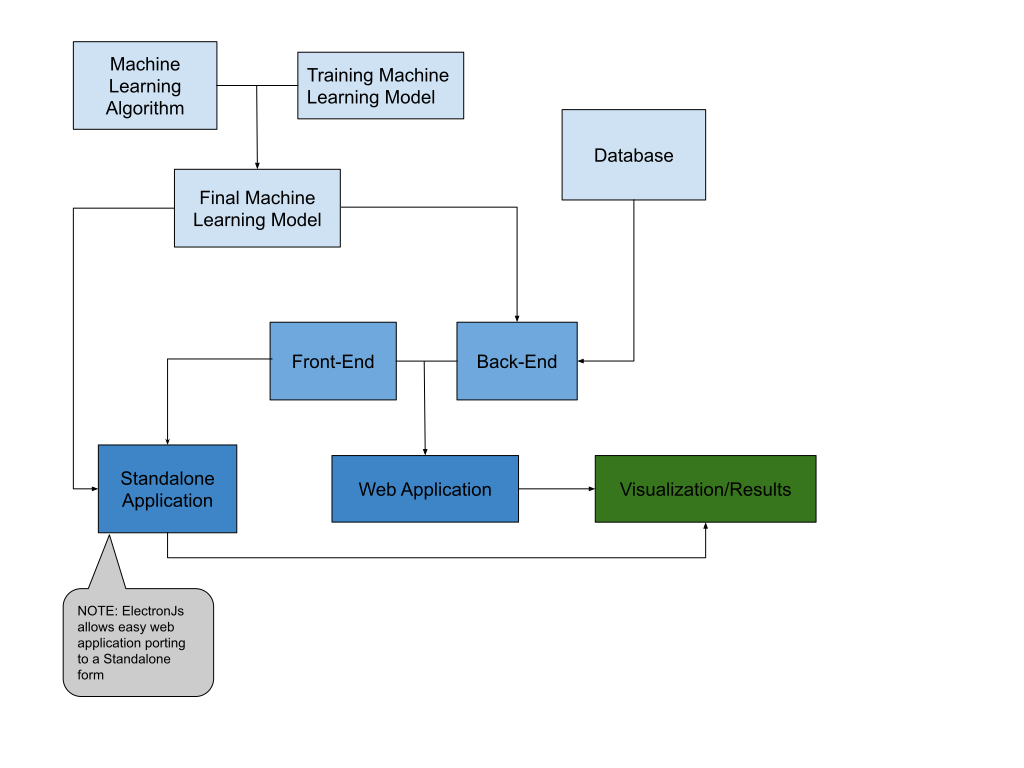
\includegraphics[width=7in]{flow_chart.png}
% where an .eps filename suffix will be assumed under latex, 
% and a .pdf suffix will be assumed for pdflatex; or what has been declared
% via \DeclareGraphicsExtensions.
\caption{Visualization of Envisioned System}
\label{fig:final_sys}
\end{figure}

\noindent To begin, we will need to create a finished machine learning model as shown in box 3. To accomplish creating the finished machine learning model, we will need to use our chosen machine learning algorithm, a Neural Network as depicted in box 1, and go through the training process of our model marked in box 2 in the figure above. The back-end depicted in box 5 will come together by connecting our MariaDB shown in box 4 with our finished machine learning model. The back-end of our web application will be developed with the Flask framework. Flask is a Python framework, which will be useful when calling our python scripts. Our front-end web framework, shown in box 6, will be developed with ReactJS, and will be responsible for the intractability of our web application. ReactJS will connect to Flask to perform necessary interactions such as button clicks, file uploads, etc, which will then fire any functions required to run our scripts. The web application, as shown in box 7, will be created from connecting the back-end to our front-end via Flask and Python. The offline fieldwork application, as shown in box 8, will use an ElectronJS GUI to incorporate all of the functionality that the web application will provide. The offline fieldwork application and web application will both be able to produce the visualizations and other results, as shown in box 9, when ran on any inputted WAV audio files. 

\section{Conclusion}
The problem that we are trying to solve is the time-consuming manual identification process of audio components in recordings from various sites in Sonoma, California. Our solution is to develop a user-friendly web application that hosts a machine learning model to automatically classify these audio components. As a stretch goal, we will also be implementing an offline fieldwork application for use on a laptop or Raspberry Pi. In order to get one step closer in making this solution a reality, we have put together this technological feasibility document. This document’s goal is to make sure that creating this project is technologically feasible. Below is a table summarizing each technical challenge we are facing, and what technology we have chosen to solve each respective challenge.\\

\noindent Proving the feasibility will continue in further testing. This analysis process allowed us to look intently at each technological challenge and research what some of the best solutions are. Our solutions to the challenges below will allow us to complete our project effectively and efficiently. Our team is confident that we will be able to produce a product that saves researchers and citizen scientists time with automated classification and an accessible user-friendly interface.

\begin{table}[H]
% increase table row spacing, adjust to taste
\renewcommand{\arraystretch}{1.3}
% if using array.sty, it might be a good idea to tweak the value of
% \extrarowheight as needed to properly center the text within the cells
\caption{Chosen Technology Summary}
\label{table_8}
\centering
% Some packages, such as MDW tools, offer better commands for making tables
% than the plain LaTeX2e tabular which is used here.
\begin{tabular}{|c|c|}
\hline
Challenge & Chosen Technology\\
\hline
Machine Learning Algorithm & Support Vector Machine\\
\hline
Training the ML Model & TensorFlow\\
\hline
Standalone App GUI & PyQT\\
\hline
Front-End Web App Framework & ReactJS\\
\hline
Back-End Web App Framework & Flask\\
\hline
Database & MariaDB\\
\hline
Visualization of Results & Plotly\\
\hline
\end{tabular}
\end{table}

% Can use something like this to put references on a page
% by themselves when using endfloat and the captionsoff option.
\ifCLASSOPTIONcaptionsoff
  \newpage
\fi

\newpage

% trigger a \newpage just before the given reference
% number - used to balance the columns on the last page
% adjust value as needed - may need to be readjusted if
% the document is modified later
%\IEEEtriggeratref{8}
% The "triggered" command can be changed if desired:
%\IEEEtriggercmd{\enlargethispage{-5in}}

% references section

% can use a bibliography generated by BibTeX as a .bbl file
% BibTeX documentation can be easily obtained at:
% http://mirror.ctan.org/biblio/bibtex/contrib/doc/
% The IEEEtran BibTeX style support page is at:
% http://www.michaelshell.org/tex/ieeetran/bibtex/
\bibliographystyle{IEEEtran}
% argument is your BibTeX string definitions and bibliography database(s)
%
% <OR> manually copy in the resultant .bbl file
% set second argument of \begin to the number of references
% (used to reserve space for the reference number labels box)
\begin{thebibliography}{3}

\bibitem{}
Abhay, ''Amazon DynamoDB - Benchmarking with Production Data \& Analysis,''\emph{Amazon DynamoDB – Benchmarking with Production Data \& Analysis, 22-Dec-2015}. [Online]. Available: http://hackpundit.com/amazon-dynamodb-benchmark-analysis-performance/. [Accessed: 06-Nov-2019].

\bibitem{}
D.~R. Amancio, C.~H. Comin, D.~Casanova, G.~Travieso, O.~M. Bruno, F.~A. Rodrigues, and L.~D. F. Costa, ''A Systematic Comparison of Supervised Classifiers,'' \emph{PLoS ONE}, vol. 9, no. 4, 2014.

\bibitem{}
J. Guerra and C. Catania, \emph{Improving the Generation of Labeled Network Traffic Datasets Through Machine Learning Techniques}. 2010.
 
\bibitem{}
E.~A. Hay and R.~Parthasarathy, ''Performance of convolutional neural networks for identification of bacteria in 3D microscopy datasets,'' \emph{PLOS Computational Biology}, vol. 14, no. 12, Mar. 2018.

\bibitem{}
M.~Herman, ''Django vs. Flask in 2019: Which Framework to Choose,''\emph{testdriven.io}, 29-Sep-2019. [Online]. Available: https://testdriven.io/blog/django-vs-flask/. [Accessed: 06-Nov-2019].

\bibitem{}
K.~Klenov, ''Python's Web Framework Benchmarks,'' \emph{Python's Web Framework Benchmarks}. [Online]. Available: https://klen.github.io/py-frameworks-bench/. [Accessed: 06-Nov-2019].

\bibitem{}
Larhmam, ''PNG.'' 19-Oct-2018.
  
\bibitem{}
''mariadb RAM usage,''\emph{MariaDB KnowledgeBase}. [Online]. Available: https://mariadb.com/kb/en/library/mariadb-ram-usage/. [Accessed: 06-Nov-2019].

\bibitem{}
B.~Morel, ''High-speed inserts with MySQL,'' \emph{Medium}, 21-Jun-2019. [Online]. Available: https://medium.com/@benmorel/high-speed-inserts-with-mysql-9d3dcd76f723. [Accessed: 06-Nov-2019].

\bibitem{}
''MySQL memory usage - Periodically need to run FLUSH TABLES or memory usage keeps growing with large-pages turned on,'' \emph{Server Fault}, 01-Mar-1964. [Online]. Available: https://serverfault.com/questions/561448/mysql-memory-usage-periodically-need-to-run-flush-tables-or-memory-usage-keeps. [Accessed: 06-Nov-2019].

\bibitem{}
''PyQt v4 - Python Bindings for Qt v4,'' \emph{Riverbank Computing} 29-Apr-2008. .

\bibitem{}
R.~Rodríguez-Pérez, M.~Vogt, and J.~Bajorath, ''Influence of Varying Training Set Composition and Size on Support Vector Machine-Based Prediction of Active Compounds,'' \emph{Journal of Chemical Information and Modeling}, vol. 57, no. 4, pp. 710–716, Oct. 2017.

\bibitem{}
M.~Shah, ''MongoDB vs MySQL: A Comparative Study on Databases,'' \emph{Insights on Latest Software Technologies - Simform Blog}, 17-Sep-2019. [Online]. Available: https://www.simform.com/mongodb-vs-mysql-databases/. [Accessed: 06-Nov-2019].

\bibitem{}
''Stack Overflow Trends,'' \emph{Stack Overflow Trends}, Stack Overflow Insights, 2019.

\bibitem{}
V.~Tkachenko, ''MySQL 5.5.8 - in search of stability,'' \emph{Percona Database Performance Blog}, 04-Jan-2011. [Online]. Available: https://www.percona.com/blog/2011/01/03/mysql-5-5-8-in-search-of-stability/. [Accessed: 06-Nov-2019].

\bibitem{}
V.~Vaintroub, ''MariaDB 5.5 performance on Windows,'' \emph{MariaDB 5.5 performance on Windows - MariaDB.org}, 09-May-2017. [Online]. Available: https://mariadb.org/mariadb-5-5-performance-on-windows/. [Accessed: 06-Nov-2019].

\bibitem{} 
A.~Verikas, E.~Vaiciukynas, A.~Gelzinis, J.~Parker, and M.~Olsson, ''Electromyographic Patterns during Golf Swing: Activation Sequence Profiling and Prediction of Shot Effectiveness,'' \emph{Sensors}, vol. 16, no. 4, p. 592, 2016.

\bibitem{}
W.~Vogels, ''Amazon DynamoDB Accelerator (DAX): Speed Up DynamoDB Response Times from Milliseconds to Microseconds without Application Rewrite.,''\emph{Amazon DynamoDB Accelerator (DAX): Speed Up DynamoDB Response Times from Milliseconds to Microseconds without Application Rewrite.}, 21-Jun-2017. [Online]. Available: https://www.allthingsdistributed.com/2017/06/amazon-dynamodb-accelerator-dax.html. [Accessed: 06-Nov-2019].

\bibitem{}
P.~Zona, ''Build Database Clusters with MongoDB,''\emph{Linode Guides & Tutorials}, 29-Jul-2019. [Online]. Available: https://www.linode.com/docs/databases/mongodb/build-database-clusters-with-mongodb/. [Accessed: 06-Nov-2019].

\end{thebibliography}

%\vfill

% Can be used to pull up biographies so that the bottom of the last one
% is flush with the other column.
%\enlargethispage{-5in}

\begin{center}
\vfill
\includegraphics[width=.1\textwidth]{images/logo.png}\\[0.5cm]
\textsc{\large IntelliChirp}
\end{center}

% that's all folks
\end{document}


